\chapter[\paperVItitle]{\texorpdfstring{%
		\paperVItitle}{%
		\paperVItitle}}
\label{ch:slightlygreedy}
\paperRemark{\paperVIref} % TODO: consider adding e.g. Reformatted for clarity

{

%\documentclass{acm_proc_article-sp}
%\documentclass{llncs}
%\documentclass[a4paper,twoside]{article}

%\usepackage[T1]{fontenc}
%\usepackage{multirow}
%\usepackage{rotating}
%\usepackage{tikz}
%\usetikzlibrary{arrows,backgrounds,patterns,shapes,decorations.markings,decorations.pathreplacing,positioning,matrix}
%\usepackage{enumitem}
%\usepackage{hyperref}
%\hypersetup{pdfborder=0 0 0}
%\usepackage{listings}
%\usepackage{booktabs}
%\usepackage{array}
%\usepackage{amsmath}
%\usepackage{amssymb}
%\usepackage{bm}
%\usepackage{calc}
%\usepackage{subcaption}
%\usepackage{multicol}

\newcommand{\cfor}{\textbf{for}}
\newcommand{\creturn}{\textbf{return}}
\newcommand{\cif}{\textbf{if}}
\newcommand{\celse}{\textbf{else}}
\newcommand{\cwhile}{\textbf{while}}
\newcommand{\crepeat}{\textbf{repeat}}

\newcounter{algcount}
\renewcommand{\thealgcount}{\arabic{algcount}}

\newcommand{\alg}[4]{
	\begin{table}[htbp]
		\centering
		\begin{tabular}{l}
			\toprule[0.4mm]
			\parbox{0.9\linewidth}{
				\refstepcounter{algcount}
				\label{#2}
				\parbox[t]{\widthof{\textbf{Algorithm \thealgcount}~--~}}{\textbf{Algorithm~\thealgcount}~--~}
				\parbox[t]{0.9\linewidth - \widthof{\textbf{Algorithm \thealgcount}~--~}}{{#1}}\vspace{.65mm}
			}\\
			\midrule[0.4mm]
			\parbox{0.9\linewidth}{#3}\\
			\midrule
			\parbox{0.9\linewidth}{{#4}}\\
			\bottomrule[0.4mm]
		\end{tabular}
	\end{table}
}

\newcommand{\algref}[1]{{Algorithm \ref{alg:#1}}}

\renewcommand{\sectionautorefname}{Section}
\renewcommand{\subsectionautorefname}{\sectionautorefname}

%\subfigtopskip=0pt
%\subfigcapskip=0pt
%\subfigbottomskip=0pt

%\begin{document}

%\title{Not so Greedy: Enhanced Subset Exploration for Nonrandomness Detectors}

%\author{Linus Karlsson \and Martin Hell \and Paul Stankovski}

% Linus Karlsson ORCID: https://orcid.org/0000-0002-6332-5078

%\institute{Dept. of Electrical and Information Technology, Lund University,\\
%P.O. Box 118, 221 00 Lund, Sweden\\
%\email{\{linus.karlsson,martin.hell,paul.stankovski\}@eit.lth.se}
%}

%\maketitle

\section*{Abstract}
Distinguishers and nonrandomness detectors are used to distinguish ciphertext from random data. In this paper, we focus on the construction of such devices using the maximum degree monomial test. This requires the selection of certain subsets of key and IV-bits of the cipher, and since this selection to a great extent affects the final outcome, it is important to make a good selection. We present a new, generic and tunable algorithm to find such subsets. Our algorithm works on any stream cipher, and can easily be tuned to the desired computational complexity. We test our algorithm with both different input parameters and different ciphers, namely Grain-128a, Kreyvium and Grain-128. Compared to a previous greedy approach, our algorithm consistently provides better results.

\section{Introduction}

Stream ciphers are symmetric cryptographic primitives which generate a pseudo-random sequence of digits, called the keystream, which is then combined with the plaintext message to produce a ciphertext. To generate the keystream, a public initialization vector (IV) and a secret key are used. It is important that an attacker cannot use the public IV to deduce information about the keystream, since this would put the encrypted message at risk.

To prevent such an attack, the key and IV are mixed during an initialization phase, before the stream cipher produces actual keystream. This initialization phase consist of a set of initialization rounds, during which the output of the cipher is suppressed.

A cipher needs to have an adequate amount of initialization rounds. Too many, and the cipher will have poor initialization performance, too few and an attacker may be able to perform an attack, e.g., a chosen-IV attack.

In this paper we will look into the design of distinguishers and nonrandomness detectors to perform cryptanalysis of different ciphers. The goal of such devices is to look at data and then determine whether the data is random data, or data from a specific cipher. Recall that for a good cipher, the keystream should be pseudo-random, so it should be hard to construct such a detection device, since data from a cipher should appear random to an outside observer.

Distinguishers and nonrandomness detectors differs in what degree of control an attacker has over the input. In a distinguisher, the key is fixed and unknown to the attacker, only the IV can be modified. In a nonrandomness detector, an attacker has more control, and can modify both key and IV bits.

The design of distinguishers and nonrandomness detectors has previously been discussed in the literature. Previous work such as \cite{englund:2007} has considered the design of such devices by using a test called the Maximum Degree Monomial (MDM) test. This test looks at statistical properties of a cipher to find weaknesses.

This test requires selection of a subset of the cipher's key and IV bits, which can be selected using, for example, a greedy algorithm, as described in ~\cite{stankovski:2010}.

We build upon this previous work and propose an improved, generalized, algorithm which outperforms the greedy algorithm in finding suitable subsets. We also implement and test our algorithm, and present new results on the stream ciphers Grain-128, Grain-128a and Kreyvium.

This paper is an extended and revised version of \cite{karlsson:2017}.
The major novelties are analysis of one more cipher (Kreyvium), a new test which investigates the effect of optimal starting subsets, and a more detailed descriptions of our algorithm.

The paper is organized as follows. In \autoref{sec:slightlygreedy:background} we present some required background, which is then used when describing our new algorithm in \autoref{sec:improvedalg}. Results are presented in \autoref{sec:results}, which is then followed by a discussion of related work in \autoref{sec:slightlygreedy:relatedwork}. \autoref{sec:slightlygreedy:conclusions} concludes the paper.

\section{Background} \label{sec:slightlygreedy:background}
In this paper we will mainly focus on the analysis of the two stream ciphers Grain-128a and Kreyvium. This selection of ciphers has been made since they share some interesting properties. They are both based on ciphers from the final eSTREAM portfolio (Grain~v1 and Trivium, respectively), but modified to have 128-bit keys. Both ciphers also update their internal state relatively slowly---a small fraction of the internal state is modified in each clock cycle. This requires both ciphers to have many initializations rounds.

For completeness, we start with a brief description of these two ciphers.
After this, in the rest of this chapter, we discuss the Maximum Degree Monomial test in more detail.

\subsection{Grain-128a}
The Grain-family of ciphers consist of a progression of multiple ciphers, starting with Grain~v1 \cite{hell:2006a}, which is included in the final eSTREAM portfolio of ciphers. This was extended into a 128-bit key version as Grain-128 \cite{hell:2006b}, and finally to the current version Grain-128a \cite{agren:2011}.

Grain-128a is a stream cipher with a 128 bit key and a 96 bit IV. It support two modes of operations, with or without authentication. For brevity, the following description will focus on the non-authenticated mode. Refer to the original paper for an extended description. The cipher is constructed with three major parts: one LFSR of size 128, one NFSR of size 128, and one pre-output function $h$ combining values from the LFSR and the NFSR. An overview of the cipher can be seen in \autoref{fig:grain128a}.

\begin{figure}
	\centering
	\begin{tikzpicture}[scale=1.0, every node/.style={scale=1.0}, node distance=2cm]
		\node[draw,minimum width=2cm] (nfsr) at (0,0) {NFSR};
		\node[right of=nfsr,inner sep=0,outer sep=0] (nfsrlfsrplus) {\LARGE $\oplus$};
		\node[draw,minimum width=2cm,right of=nfsrlfsrplus] (lfsr) {LFSR};
		
		\node[draw,below=0.5cm of nfsrlfsrplus] (h) {$h$};
		\node[below=0.5cm of h,inner sep=0,outer sep=0] (hplus) {\LARGE $\oplus$};
		
		\draw[->] (lfsr.west) -- (nfsrlfsrplus.east);
		\draw[->] (nfsrlfsrplus.west) -- (nfsr.east);
		
		\draw[->] (nfsr.south) |- (h.west);
		\draw[->] (lfsr.south) |- (h.east);
		
		\coordinate (nfsrsouth2) at ([xshift=-0.5cm]nfsr.south);
		\coordinate (lfsrsouth2) at ([xshift=0.5cm]lfsr.south);
		\draw[->] (nfsrsouth2) |- (hplus.west);
		\draw[->] (lfsrsouth2) |- (hplus.east);
		\draw[->] (h.south) -- (hplus.north);
		\draw[->] (hplus.south) -- ++(0cm,-0.5cm) node[midway,right] {$z$};
		
		% feedback functions.
		\coordinate[above=0.5cm of nfsrlfsrplus] (aboveplus);
		\draw[->] (nfsr.north) -- (aboveplus -| nfsr.north) -- (aboveplus) node[midway,above] {$g$} --  (nfsrlfsrplus.north);

		\coordinate[right=0.5cm of lfsr.east] (lfsrr);
		\draw[->] (lfsr.north) -- (aboveplus -| lfsr.north) -- (aboveplus -| lfsrr) node[midway,above] {$f$} -- (lfsrr) -- (lfsr.east);
	\end{tikzpicture}
	\caption{Overview of Grain-128a}
	\label{fig:grain128a}
\end{figure}

The functions $f(x)$ and $g(x)$ are the feedback functions for the LFSR and the NFSR respectively. They are defined as follows:
\[
f(x) = 1 + x^{32} + x^{47} + x^{58} + x^{90} + x^{121} + x^{128}
\]
and
\begin{align*}
	g(x) &= 1 + x^{32} + x^{37} + x^{72} + x^{102} + x^{128} + x^{44}x^{60} + x^{61}x^{125} + x^{63}x^{67} \\
		 &+ x^{69}x^{101} + x^{80}x^{88} + x^{110}x^{111} + x^{115}x^{117} + x^{46}x^{50}x^{58} \\
		 &+ x^{103}x^{104}x^{106} + x^{33}x^{35}x^{36}x^{40}
\end{align*}

The function $h(x)$ is defined as follows, where $s_i$ and $b_i$ correspond to the $i$th state variable of the LFSR and the NFSR respectively: 
\[
h = b_{12}s_{8} + s_{13}s_{20} + b_{95}s_{42} + s_{60}s_{79} + b_{12}b_{95}s_{94}
\]
Finally, the output $z$ from the cipher is constructed as:
\[
z = h + s_{93} + b_{2} + b_{15} + b_{36} + b_{45} + b_{64} + b_{73} + b_{89}
\]

The initialization of the cipher is as follows. At first the NFSR is filled with the 128 key bits, and then the LFSR is filled with the 96 IV-bits. The remaining 32 bits of the LFSR are filled with ones, except the final bit which is set to zero. After this, the cipher is clocked 256 times, during which the output is suppressed and instead fed back and XORed with the input to both the NFSR and LFSR. After this, the cipher is ready and starts to produce keystream.

\subsection{Kreyvium}
Kreyvium \cite{canteaut:2016} is based on another eSTREAM finalist, namely Trivium \cite{canniere:2006}. Trivium is notable for its simplistic design. It has an 80 bit key and an 80 bit IV. The authors of Kreyvium modifies the construction by increasing this to 128 bit for both the key and the IV.

Kreyvium's internal state consists of five different registers, of sizes 93, 84, 111, 128, and 128 bits. In the following brief description, we will call them $a$, $b$, $c$, $IV^*$, and $K^*$, respectively. The first three registers are the same as in Trivium, while the latter two are added in Kreyvium. An overview of the cipher can be found in \autoref{fig:kreyvium}.

\begin{figure}
	\centering
	\begin{tikzpicture}[scale=1.0, every node/.style={scale=1.0}, node distance=1cm]
		\node[draw,minimum width=2cm,minimum height=0.5cm] (ivstar) at (0,0) {$IV^*$};
		\node[draw,minimum width=2cm,minimum height=0.5cm,below=of ivstar] (a) {$a$};
		\node[draw,minimum width=2cm,minimum height=0.5cm,below=of a] (b) {$b$};
		\node[draw,minimum width=2cm,minimum height=0.5cm,below=of b] (c) {$c$};
		\node[draw,minimum width=2cm,minimum height=0.5cm,below=of c] (kstar) {$K^*$};
		
		\node[right=3cm of b,outer sep=0,inner sep=0] (zplus) {\Large $\oplus$};
		\node[left=0.3cm of zplus,outer sep=0,inner sep=0] (zplusl) {\Large $\oplus$};
		\node[right=1cm of a,outer sep=0,inner sep=0] (aplus) {\Large $\oplus$};
		\node[right=1cm of b,outer sep=0,inner sep=0] (bplus) {\Large $\oplus$};
		\node[right=1cm of c,outer sep=0,inner sep=0] (cplus) {\Large $\oplus$};
		
		\coordinate[right=0.3cm of aplus] (aplusr);
		\coordinate[above right=0.4cm and 0.2cm of aplusr] (aplusr2);
		\coordinate[right=0.4cm of bplus] (bplusr);
		
		% z generation
		\draw[->] (zplus.east) -- ++(0.5cm,0) node[midway,above] {$z$};
		\draw[->] (zplusl.east) -- (zplus.west);
		
		\coordinate[above=0.3cm of a] (aabove);
		\coordinate[above=0.3cm of b] (babove);
		\coordinate[above=0.3cm of c] (cabove);
		\coordinate[above=0.3cm of kstar] (kstarabove);
		\draw[->] (a.north) -- (aabove) -- (aabove -| zplus.north) -- (zplus.north);
		\draw[->] (b.north) -- (babove) -- (babove -| zplusl.north) -- (zplusl.north);
		\draw[->] (c.north) -- (cabove) -- (cabove -| zplusl.south) -- (zplusl.south);
		\draw[->] (kstar.north) -- (kstarabove) -- (kstarabove -| zplus.south) -- (zplus.south);
		
		% various helpers.
		\coordinate[below=0.3cm of a] (abelow);
		
		% feedback for K*
		\coordinate[right=0.5cm of kstar] (kstarr);
		\coordinate[below=0.3cm of kstar] (kstarbelow);
		\draw[->] (kstar.south -| kstarbelow) -- (kstarbelow) -- (kstarbelow -| kstarr) |- (kstar.east);

		% feedback for IV*
		\coordinate[below=0.3cm of ivstar] (ivstarbelow);
		\coordinate[right=0.5cm of ivstar] (ivstarr);
		\draw[->] (ivstar.south -| ivstarbelow) -- (ivstarbelow) -- (ivstarbelow -| ivstarr) |- (ivstar.east);

		% feedback for b
		\draw[->] (bplus) -- (b.east);
		
		\coordinate[below left=0.1cm and 0.1cm of ivstarbelow] (ivstarbelow2);
		\coordinate[below left=0.1cm and 0.1cm of abelow] (abelow2);
		\coordinate[below=0.3cm of b] (bbelow);
		\draw[->] (a.south -| abelow2) -- (abelow2) -- (abelow2 -| bplus.north) -- (bplus.north);
		\draw[->] (b.south) -- (bbelow) -- (bbelow -| bplus.south) -- (bplus.south);
		\draw[->] (ivstar.south -| ivstarbelow2) -- (ivstarbelow2) -- (ivstarbelow2 -| bplusr) -- (bplusr) -- (bplus.east);
		
		% feedback for c
		\draw[->] (cplus) -- (c.east);
		
		\coordinate[below left=0.1cm and 0.1cm of bbelow] (bbelow2);
		\coordinate[below=0.3cm of c] (cbelow);
		\draw[->] (b.south -| bbelow2) -- (bbelow2) -- (bbelow2 -| cplus.north) -- (cplus.north);
		\draw[->] (c.south -| cbelow) -- (cbelow) -- (cbelow -| cplus.south) -- (cplus.south);
		
		% feedback for a
		\draw[->] (aplus) -- (a.east);
		
		\coordinate[below left=0.1cm and 0.1cm of cbelow] (cbelow2);
		\coordinate[below left=0.1cm and 0.1cm of kstarbelow] (kstarbelow2);
		\draw[->] (a.south -| abelow) -- (abelow) -- (abelow -| aplus.south) -- (aplus.south);
		\draw[->] (c.south -| cbelow2) -- (cbelow2) -- (cbelow2 -| aplusr) -- (aplusr) -- (aplus.east);
		\draw[->] (kstar.south -| kstarbelow2) -- (kstarbelow2) -| (aplusr2) -| (aplus.north);
	\end{tikzpicture}
	\caption{Overview of Kreyvium}
	\label{fig:kreyvium}
\end{figure}

Following the notation of the original paper, the registers $a$, $b$, and $c$ are numbered $s_1, \ldots, s_{93}$, followed by  $s_{94}, \ldots, s_{177}$, and finally $s_{178}, \ldots, s_{288}$, respectively. Then the output $z$ can be expressed as:

\[
z = s_{66} + s_{93} + s_{162} + s_{177} + s_{243} + s_{288} + K^*_0
\]

For every clock, each LFSR is shifted one step, and the following values are shifted in for each register:
\begin{align*}
s_1 &= s_{243} + s_{288} + K^*_0 + s_{286}s_{287} + s_{69} \\
s_{94} &= s_{66} + s_{93} + s_{91}s_{92} + s_{171} + IV^*_0 \\
s_{178} &= s_{162} + s_{177} + s_{175}s_{176} + s_{264} \\
K^*_{127} &= K^*_0 \\
IV^*_{127} &= IV^*_0 \\
\end{align*}

The initialization of the ciphers is as follows. The $a$ register is initialized with the first 93 key bits. The $b$ register is intialized with the first 84 IV bits. The $c$ register is initialized with the remaining IV bits, followed by all ones, except the final bit which is a zero. The $K^*$ register is filled with the key, and the $IV^*$ register is filled with the IV. After this the cipher is clocked 1152 times, during which the output is suppressed. After this, the cipher starts generating keystream.

\subsection{Maximum Degree Monomial Test}
The maximum degree monomial test was first presented in \cite{englund:2007} and described a clean way to detect nonrandomness by looking at the cipher output.

Considering an arbitrary stream cipher, we can consider it as a black box with two inputs, and one output. The input is the key $K$ and the initialization vector (IV) $V$ respectively, while the output is the generated keystream. We consider the concatenation of the key $K$ and the IV $V$ as a boolean space $B$ of dimension $b=|K| + |V|$.

Any Boolean function $g$ over a boolean space $B$ can be described by its Algebraic Normal Form (ANF)
\[
g(x_1, x_2, \ldots, x_b) = c_0 + c_1 x_1 + c_2 x_2 + \ldots + c_m x_1 x_2 \ldots x_b
\]
where the coefficients $c_i$ are either 0 or 1, thus describing if the term is included in the ANF or not. For the function $g$ above, the last term with coefficient $c_m$ describes the maximum degree monomial. If $c_m$ is zero, we say that the maximum degree monomial does not exist, while if $c_m$ is 1, we say it does exist. We note that for a randomly chosen Boolean function $g$, we would expect the maximum degree monomial to appear with a probability of $\frac{1}{2}$.

We are interested in finding out whether or not the maximum degree monomial exists in the ANF of the Boolean function of the first keystream bit. The rationale behind this is that intuitively, the maximum degree monomial tells us something about the mixing of the input to the cipher. Since the maximum degree monomial is the product of all inputs of the Boolean function, we expect to see it only if all inputs have been mixed.

It is well known that according to the Reed-Muller transform, the coefficient of the maximum degree monomial can be found simply by XORing all the entries in the truth table of a Boolean function as
\begin{align}
\bigoplus_{\bm{x} \in \{0,1\}^b}^{} g(\bm{x}) \label{eq:reedmuller}
\end{align}
where $g(\bm{x})$ is a Boolean function. Thus all possible values for the input set is generated, and for each input value the function is evaluated.

We will use this test to analyze the required amount of initialization rounds of a stream cipher. The designers of a stream cipher need to select how many initialization rounds to perform: too few, and it may be possible to attack the cipher, too many, and the performance hit will be large.

If we consider the first bit of keystream from a stream cipher as a Boolean function, we can choose to sum over this function in Equation~\ref{eq:reedmuller} above. The input $\bm{x}$ would then correspond to the input set of key and IV bits.

Instead of only looking at the first bit of real keystream, the idea can be extended such that a modified version of the cipher is considered. In the modified version, we also look at the cipher's output during its initialization rounds, output which is normally suppressed. Assuming a cipher with $l$ initialization rounds, we denote the $i$th initialization round output function as $f_i(\bm{x})$, thus giving us a vector
\[
\underbrace{f_1(\bm{x}), f_2(\bm{x}), \ldots, f_l(\bm{x})}_{l \text{ functions}} \,.
\]

Thus, instead of only looking at the ANF and finding the maximum degree monomial of a single function ($z_0$ before), we now look at $l$ different boolean functions, and for each of the functions, we find the coefficient of the maximum degree monomial. Such a sequence would have a format like
\[
\underbrace{01100101\ldots101}_{l\text{ coefficients}}
\]
where each individual bit is the maximum degree monomial coefficient for its corresponding function $f_i$.
We call this sequence of coefficients the \emph{maximum degree monomial signature}, or MDM signature, following the terminology in \cite{stankovski:2010}.

Since the keystream is a pseudo-random sequence of digits, the keystream produced by an ideal stream cipher should, to an outside observer, be indistinguishable from a random stream of bits. This means that if we look at each output bit function $f_i(\bm{x})$, it should appear to be a random function $f_i: B \rightarrow \{0,1\}$. As noted earlier, for a random Boolean function, we expect the maximum degree monomial to exist with probability $\frac{1}{2}$. Therefore, we expect the coefficients 0 and 1 to appear with equal probability, and for an ideal cipher, we expect to see a random-looking MDM signature.

However, if the input space $B$ is large, clearly the construction of a MDM signature will result in too many initialization of the cipher to be feasible. Therefore, we can only consider a subset $S$ of the input space $B$. The remaining part, $B \setminus S$, is set to some constant value, in this paper we selected it to be zero.

% XXX: subsection rewritten.
\subsection{Finding the Subset $S$}
The selection of the subset $S$ turns out to be a crucial part of the MDM test. We will soon see that depending on the choice of $S$, the resulting MDM signature will vary greatly.

Consider a subset $S$ of key and IV bits for the stream cipher Grain-128a \cite{agren:2011}. Choosing $S$ as key bit 23, and IV bits 47, 53, 58, and 64, we get the following MDM signature:

\[
\underbrace{000\ldots 000}_{\text{187 zeros}}111\ldots
\]

Looking at the initial sequence of 187 adjacent zeros, out first conclusion is that this does not appear to be a random-looking sequence. After this, we will however start to see ones and zeros in a more mixed fashion. From this we can intuitively say the it appears as if 187 initialization rounds are not enough. However, Grain-128a is designed with 256 initialization rounds in a non-modified implementation, and thus it appears as if the designers have chosen a sufficiently high amount of initialization rounds.

To more concisely describe the result above, we state that \emph{we find nonrandomness in 187 out of 256 initialization rounds}. We will use this terminology throughout the paper. Worth noting is also that this is a nonrandomness result, since we have included both key and IV bits as a part of the subset $S$.

From the description above, it should not come as a surprise that our goal now is to maximize the length of the initial sequence of zeros we can find in the MDM signature. The ultimate goal is of course to find nonrandomness in \emph{all} initialization rounds, at which point it may be interesting to look for it in the actual keystream of an unmodified cipher.

The selection of what bits to include from $B$ into the subset $S$ is important. The composition of $S$ will greatly influence the resulting MDM signature. Four examples can be found in \autoref{tbl:sgrain128a}.

%The subset $S$ plays a crucial role here. Its composition affects the resulting MDM signature to a great extent. Consider the two examples for Grain-128a found in \autoref{tbl:sgrain128a}.

\begin{table}[h]
	\caption{The number of initial zeros in the MDM signature for four different subsets $S$ for Grain-128a}
    \centering
	\begin{tabular}{llr}
		\toprule
		$K$ & $IV$ & rounds out of 256 \\
		\midrule
		$\{  \}$ & $\{ 1,2,3,4,5 \}$ & $107$ \\
		$\{  \}$ & $\{ 91,92,93,94,95 \}$ & $124$ \\
		$\{ 23 \}$ & $\{ 47,53,58,64 \}$ & $187$ \\
		$\{ 1,2,3,4,5 \}$ & $\{  \}$ & $109$ \\
		\bottomrule
	\end{tabular}
	\label{tbl:sgrain128a}
\end{table}

% [Sun 16:24:26, 0 days  0 h  0 min  0 sec] Bit set size  5  ->  109 / 256 zero bits = 42.58%, xor = 00000000000000000000000000607839B8EFD040384DB9C1FF91400F6CAF64FE, Key bit set = {  1,  2,  3,  4,  5 }, IV bit set = { }
% [Sun 16:25:40, 0 days  0 h  0 min  0 sec] Bit set size  5  ->  124 / 256 zero bits = 48.44%, xor = 00000000000000000000000000000030A1BA20CA751C9482B7CADB9AA01739B5, Key bit set = { }, IV bit set = { 95, 94, 93, 92, 91 }
% [Sun 16:23:59, 0 days  0 h  0 min  0 sec] Bit set size  5  ->  187 / 256 zero bits = 73.05%, xor = 0000000000000000000000000000000000000000000000F88B6C7D59A8A5A2D6, Key bit set = { 23 }, IV bit set = { 47, 53, 58, 64 }


From the table above, we can clearly see that the choice of $S$ is crucial. For these examples, we have selected a subset size of five, i.e. $|S|=5$, and included both key and/or IV bits in $S$. The third row, where we find 187 consecutive zeros, is actually the optimal result for a subset of size 5. Calculating the optimal result is however not feasible as the subset grows larger. For the general case, where the input space is $B$ and the subset is $S$, we would have to test $\binom{|B|}{|S|}$ combinations. Again, using Grain-128a as an example, that would correspond to $\binom{224}{|S|}$ combinations, since Grain-128a has 96 IV bits and 128 key bits.

% XXX: rewritten.
\subsection{Greedy Approach} \label{sec:greedybackground}
Since the selection of the subset $S$ is important, we now turn our attention to algorithms used to construct such a subset. Previous work, such as \cite{stankovski:2010}, has proposed to use a greedy algorithm to find such a subset. The greedy approach can, in short, be described through the following steps, which results in a subset of a desired size:

\begin{enumerate}
	\item Find an optimal starting subset of a small size (possibly empty, making this step optional)
	\item Add the $n$ bits which together produce the highest number of zero rounds to the current subset. \label{itm:greedyiter}
	\item Repeat step~\ref{itm:greedyiter} until a subset of the wanted size $m$ is found.
\end{enumerate}

To make the algorithm even clearer, consider the following example where we start with the optimal subset of size five described earlier in \autoref{tbl:sgrain128a}. A few steps of the greedy algorithm, with $n=1$, would then look like this:
\begin{center}
	\begin{tikzpicture}[scale=1.0, every node/.style={scale=1.0}]
	\matrix (m)[matrix of nodes,column sep=3mm,row sep=0mm,align=left,nodes={anchor=base west},ampersand replacement=\&]
	{
		\node{$i_0:$}; \& \node{$K = \{23\}$}; \& $IV = \{47, 53, 58, 64\}$ \\
		\node{$i_1:$}; \& \node{$K = \{23\}$}; \& $IV = \{47, 53, 58, 64, 12\}$ \\
		\node{$i_2:$}; \& \node{$K = \{23, 72\}$}; \& $IV = \{47, 53, 58, 64, 12\}$ \\
		\node{$i_3:$}; \& \node{$K = \{23, 72, 31\}$}; \& $IV = \{47, 53, 58, 64, 12\}$ \\
		\node{$i_4:$}; \& \node{$K = \{23, 72, 31, 107\}$}; \& $IV = \{47, 53, 58, 64, 12\}$	\\
	};
	\end{tikzpicture}
\end{center}

The algorithm, in iteration $i_0$ starts with the optimal subset of size 5. In iteration $i_1$ all possible remaining bits are tried, and the best bit, i.e. the one giving the longest initial sequence of zeros, is selected and included in the subset, in this case IV bit 12. The algorithm then repeat the same step for all remaining iterations until a subset of the desired size is found, in this example $|S|=9$.

This greedy algorithm has the same drawbacks as for greedy algorithms in general---they may not find the global optimum, but rather get stuck in a local optima, thus resulting in a poor selection of $S$.

% XXX: rewritten
\section{Improved Algorithm} \label{sec:improvedalg}

Considering the possible issues of the greedy algorithm presented in the previous section, we propose a more general solution which can achieve better results. The main idea to solve this efficiency problem is to extend the na\"{i}ve greedy algorithm to examine more possible paths.

Rather than only considering the single best candidate in each iteration, our improved algorithm will store and explore a multitude of possible paths.
The rationale behind this approach is that the second best candidate in one iteration may be better in the following iteration of the algorithm, when more bits are to be added.

\begin{figure}[t]
	\begin{center}
		\tikzstyle{vecArrow} = [thick, decoration={markings,mark=at position
			1 with {\arrow[semithick]{open triangle 60}}},
		double distance=1.4pt, shorten >= 5.5pt,
		preaction = {decorate},
		postaction = {draw,line width=1.4pt, white,shorten >= 4.5pt}]
		\begin{tikzpicture}
		[node distance=.5cm,auto,>=latex',scale=0.9, every node/.style={scale=0.9},
		brcb/.style = {decoration={brace,pre=moveto,pre length=10pt,post=moveto,post length=10pt,raise=0.5mm, amplitude=3pt}, decorate},
		%		shorten <>/.style = {shorten >=#1pt, shorten <=#1pt},
		brcbl/.style = {decoration={brace,pre=moveto,pre length=10pt,post=moveto,post length=10pt,raise=0.5mm, amplitude=3pt}, decorate},
		%		shorten <>/.style = {shorten >=#1pt, shorten <=#1pt},
		brcbm/.style = {decoration={brace,pre=moveto,pre length=5pt,post=moveto,post length=5pt,raise=0.5mm,mirror,amplitude=3pt}, decorate},
		%		shorten <>/.style = {shorten >=#1pt, shorten <=#1pt}
		]
		\def\thecolsep{2pt}
		% Ugly hack to get a consistent image size.
		%\draw[use as bounding box] (-1.8,-4) rectangle (11.5,4);
		% i=0
		\node (A) {
			$\arraycolsep=\thecolsep \left[\begin{array}{ccc}
			2 &    ,   & 16 \\
			8 &    ,   & 43 \\
			32 &    ,   & 69 \\
			%				 9 &    ,   & 12 \\
			& \vdots & \\
			\end{array}\right]$
		};
		\draw [brcbm] (A.north west) -- (A.south west) node[midway,xshift=-2.1cm] {\small $\ldots k_{i-1} \alpha_{i-1}$};
		%\draw [brcb]  (A.north west) -- (A.north east) node[midway,yshift=0.2cm] {$n_{i-1}$};
		
		% i=1
		\node[above right=0.5cm and 1cm of A] (B1) {
			$\arraycolsep=\thecolsep \left[\begin{array}{ccccc}
			2 & , & 16 &   ,    & 86 \\
			2 & , & 16 &   ,    & 55 \\
			&   &    \vdots \\
			\end{array}\right]$
		};
		\draw [brcbm] (B1.north west) -- (B1.south west) node[midway,xshift=-0.7cm] {$k_i$};
		\draw [brcbl]  (B1.north) -- (B1.north east) node[midway,xshift=0pt,yshift=0.1cm] {$n_i$};
		
		\node[right=1cm of A] (B2) {
			$\arraycolsep=\thecolsep \left[\begin{array}{ccccc}
			8 & , & 43 &   ,    & 54 \\
			8 & , & 43 &   ,    & 27 \\
			&   &    \vdots \\
			\end{array}\right]$
		};
		\draw [brcbm] (B2.north west) -- (B2.south west) node[midway,xshift=-0.7cm] {$k_i$};
		\draw [brcbl]  (B2.north) -- (B2.north east) node[midway,xshift=0pt,yshift=0.1cm] {$n_i$};
		
		\node[below right=0.5cm and 1cm of A] (B3) {
			$\arraycolsep=\thecolsep \left[\begin{array}{ccccc}
			32 & , & 69 &   ,    & 5 \\
			32 & , & 69 &   ,    & 8 \\
			&   &    \vdots \\
			\end{array}\right]$
		};
		\draw [brcbm] (B3.north west) -- (B3.south west) node[midway,xshift=-0.7cm] {$k_i$};
		\draw [brcbl]  (B3.north) -- (B3.north east) node[midway,xshift=0pt,yshift=0.1cm] {$n_i$};
		
		% Arrows to Bx
		\coordinate (Afirst) at ([xshift=-0.2cm,yshift=-0.25cm]A.north east);
		\coordinate (Asecond) at ([yshift=-0.40cm]Afirst);
		\coordinate (Athird) at ([yshift=-0.40cm]Asecond);
		\draw[->,thick] (Afirst) -- (B1.west);
		\draw[->,thick] (Asecond) -- (B2.west);
		\draw[->,thick] (Athird) -- (B3.west);
		
		% sort, merge, and reduce step.
		\node[right=2.6cm of B2] (BM) {
			$\arraycolsep=\thecolsep \left[\begin{array}{ccccc}
			8 & , & 43 & , & 54 \\
			2 & , & 16 & , & 86 \\
			8 & , & 43 & , & 27 \\
			&   &   \vdots \\
			\end{array}\right]$
		};
		\draw [brcbm] (BM.north west) -- (BM.south west) node[midway,xshift=-2.8cm] {\small $\ldots k_{i-1} \alpha_{i-1} k_i \alpha_i$};
		
		\draw[vecArrow] ([yshift=1.2cm]B2.east) --  node {\scriptsize merge, sort, reduce} ([yshift=1.2cm]BM.west);
		\end{tikzpicture}
	\end{center}
	\caption{One step of our improved algorithm \cite{karlsson:2017}}
	\label{fig:overview}
\end{figure}

Increasing the number of explored candidates in each step of the algorithm will of course increase the computational complexity of the algorithm. We will, however, later derive the an expression for calculating the total computational effort required for certain parameters. In this way, we can easily estimate the computation time required.

The algorithm can briefly be described as follows:
The algorithm starts with either an optimal set of candidates, or an empty set. Each member of set is called a candidate, and every candidate is in itself a subset of key and IV-bits. For each candidate, the algorithm now tries to find the best bits to add, to maximize the initial sequence of zeros in the resulting MDM signature. This is done for each of the original candidates, which means that this generates several new sets of candidates. If this is repeated, the number of candidates clearly will grow to unmanageable numbers. Therefore, the algorithm limits the resulting set of new candidates with some factor.

A more formal and detailed description of the algorithm is described below. A description in pseudo-code can be found in \algref{slightlygreedy} and \algref{findbest}. The algorithm is parametrized by three different parameter vectors: $\bm{\alpha}$, $\bm{k}$, and $\bm{n}$. We also provide a graphical presentation of one iteration of the algorithm in \autoref{fig:overview}, which we will refer to in the more detailed, textual, description below:

\begin{enumerate}
	\item Consider a set of candidates from a previous iteration, or from an optimal starting set. If this is the first iteration, it is also possible to start with a completely empty subset of key and IV bits. In that case the algorithm starts with a single candidate, where the MDM signature is calculated with all key and IV bits set to zero. \label{itm:improvedalgfirst}
	\item For each candidate in the list, the algorithm adds the $k_i$ best $n_i$ new bits and store them in a new list. Note that there now exists one such new list for each candidate in the original list.
	\item Merge all lists, sorting by the number of zeros in the MDM signature. This gives a list of $k_0\alpha_0\ldots k_{i-1} \alpha_{i-1} k_i$ items, since there were $k_0\alpha_0\ldots k_{i-1} \alpha_{i-1}$ candidates in the beginning of this iteration, and each one has now resulted in $k_i$ new candidates.
	\item Finally, reduce the size of this merged list with the factor $\alpha_{i}$ ($0 < \alpha_i \le 1.0$), limiting the size of the combined list to $k_0\alpha_0\ldots k_{i-1} \alpha_{i-1} k_i \alpha_i$ items. If this step is omitted, or if $\alpha_i$ is set to $1.0$, the number of candidates will grow exponentially.
	\item Repeat from step~\ref{itm:improvedalgfirst} until a subset $S$ of the wanted size has been found.
\end{enumerate}

We earlier stated that this improved algorithm was a more general approach compared to the na\"{i}ve greedy algorithm described in \autoref{sec:greedybackground}. Using our new, improved algorithm and its input parameters $\bm{k}$, $\bm{n}$, and $\bm{\alpha}$, we can express the previous greedy algorithm's behavior as a specific set of input parameters, namely $\bm{\alpha} = [1.0, 1.0, \ldots])$, $\bm{k} = [1, 1, \ldots]$, and $\bm{n} = [n, n, \ldots]$. Thus our improved algorithm is a generalization of the previous algorithm, with many more degrees of freedom.

\alg{SlightlyGreedy \cite{karlsson:2017}}{alg:slightlygreedy}
{
	\textbf{Input:} key $K$, IV $V$, bit space $B$, maximum subset size $m$, vector $\bm{k}$, vector $\bm{n}$, vector $\bm{\alpha}$ \\
	\textbf{Output:} subset $S$ of size $m$.
}
{
	$S_0 = \{\emptyset\}$ \\
    /* The set $S_0$ contains a single empty subset */\\
	\cfor{} (each $i \in \{0, \ldots, m - 1\}$) \{ \\
	\indent\hspace{0.4cm}\cfor{} (each $c \in S_i$) \{ \\
	\indent\hspace{0.8cm}    $L_c$ = FindBest($K, V, B, c, k_i, n_i$); \\
	\indent\hspace{0.4cm}\} \\
	\indent\hspace{0.4cm}$S_{i+1}$ = concatenate(all $L_c$ from above); \\
	\indent\hspace{0.4cm}sort $S_{i+1}$ by the number of consecutive zeros in the MDM signature; \\
	\indent\hspace{0.4cm}reduce the number of elements in $S_{i+1}$ by a factor $\alpha_i$; \\
	\} \\
	\creturn{} $S_m$;
}

\alg{FindBest \cite{karlsson:2017} }{alg:findbest}
{
	\textbf{Input:} key $K$, IV $V$, bit space $B$, current subset $c$, number of best subsets to retain $k$, bits to add $n$ \\
	\textbf{Output:} $k$ subsets each of size $|c| + n$.
}
{
	/* let $\binom{S}{k}$ denote the set of all $k$-combinations of a set $S$. */ \\
	\\
	$S = \emptyset$; \\
	\cfor{} (each $n$-tuple $\{b_1, \ldots, b_n\} \in \binom{B\setminus c}{n}$) \{ \\
	\indent\hspace{0.4cm}$z = $ number of initial zeros using subset $c \cup \{b_1, \ldots, b_n\}$; \\
	\indent\hspace{0.4cm}\cif{} ($z$ is among the $k$ highest values) \{ \\
	\indent\hspace{0.8cm}    add $c \cup \{b_1, \ldots, b_n\}$ to $S$; \\
	\indent\hspace{0.8cm}    reduce $S$ to $k$ elements by removing element with lowest $z$; \\
	\indent\hspace{0.4cm}\} \\
	\} \\
	\creturn{} $S$;
}

\subsection{Computational Cost}
The improved algorithm may have a greater computation cost compared to the previous greedy algorithm, because it considers more candidates. The computational cost will depend on the input parameter vectors, since they affect the amount of candidates explored.

The total computational cost $C$ is expressed as the number of initializations required. The cost is expressed according to the following function, from \cite{karlsson:2017}, where $c$ is the number of iterations required ($c=|\bm{k}|=|\bm{n}|=|\bm{\alpha}|$), and $b$ is the bit space size $b=|B|$.

\begin{align}
C(b, c, \bm{k}, \bm{n}, \bm{\alpha}) = 
\sum_{i=0}^{c-1} \left[ 2^{\sum_{j=0}^{i} n_j} \binom{b - \sum_{j=0}^{i-1} n_j}{n_i} \prod_{j=0}^{i-1} k_j \alpha_j \right]
\label{eq:complexity}
\end{align}

The expression can be derived using combinatorics. In the expression, the power of two is related to the size of the different subsets $S$---a large subset requires more initializations of the cipher. The binomial coefficient is the number of possible subsets we can form given the current iteration's $n_i$. Finally, the final product is needed because the algorithm reduces the number of candidates in each iteration using the factors in $\bm{\alpha}$.
Clearly, in practice, the actual running time is also dependent on other factors, such as the cipher we are running the algorithm on.

As a special case of the expression in \autoref{eq:complexity}, an expression for the previous greedy algorithm can be derived. Recall that this algorithm had a constant $n$, and since it only considered the best candidate in each iteration, both $\bm{k}$ and $\bm{\alpha}$ are all ones. Under these constraints, the expression can more concisely be given as \cite{karlsson:2017}:

\begin{align}
C(b, c, n) = \sum_{i=0}^{c-1} \left[ 2^{n(i+1)} \binom{b - n \cdot i}{n} \right]
\label{eq:complexitygreedy}
\end{align}


%or if one-indexed:
%\begin{align}
%C(b, c, \bm{k}, \bm{n}, \bm{\alpha}) = \sum_{i=1}^{c} \left[ 2^{\sum_{j=1}^{i} n_j} \binom{b - \sum_{j=1}^{i-1} n_j}{n_i} \prod_{j=1}^{i-1} k_j \alpha_j \right]
%\label{eq:complexityoneindex}
%\end{align}

\section{Results} \label{sec:results}
To get any results from our proposed algorithm, the choice of parameters must first be discussed. The algorithm is parametrized by the parameter vectors $\bm{k}$, $\bm{n}$, and $\bm{\alpha}$. In this section we will explore and investigate how the choice of parameters affect the final result of our algorithm. These new results will be compared to the previous greedy algorithm as a baseline.

The greedy algorithm only had one degree of freedom, $n$, while the improved algorithm has many more. We have performed a significant amount of simulations, on several different ciphers, to be able to present results on how the choice of parameters affect the results of the algorithm.

The tests have been performed on the stream ciphers Grain-128a \cite{agren:2011}, Kreyvium \cite{canteaut:2016}, and to some extent Grain-128 \cite{hell:2006b}. For reference, the exact parameters used for each result presented below are available in the Appendix of this paper.

\subsection{Tuning the Greediness} \label{sec:tuninggreedy}

To get a feeling for how the different parameters affect the result, we start by varying the two parameter vectors $\bm{k}$ and $\bm{\alpha}$, while keeping $\bm{n}$ consistent, and equal to an all-one vector.
While $\bm{k}$ and $\bm{\alpha}$ gives almost unlimited possibilities, we have opted for the following simulation setup.

For every test case, a given iteration $i$ will have the same amount of candidates, which makes the computational complexity identical between the different test cases. The input vectors $\bm{k}$ and $\bm{\alpha}$ will of course be different for the different test cases, which in turn mean that even if the amount of candidates is the same, the actual candidates will vary between the tests. By designing the test this way, we wish to investigate how this difference in candidate selection affect the final result of the algorithm.

Recall that $k_i$ govern how many new candidates we generate from a previous iteration's subsets. A high $k_i$ and low $\alpha_i$ means that we may end up with several candidates that have the same ``stem'', i.e. they have the same origin list. If we lower $k_i$ and instead increase $\alpha_i$ we will get a greater mix of different stems, while still maintaining the same amount of candidates for the iteration---in a sense the greediness of the algorithm is reduced. Thus, we want to test some different tradeoffs between the two parameters. In the results below, we name the different test cases as a percentage value of the total amount of candidates for each round. As an example, if the total number of candidates in a given round is 1000, we could select a $k_i$ of 200, and a corresponding $\alpha_i$ of $0.005$, which gives us 1000 candidates for the next round as well. We call this particular case \emph{20 \%-k} since $k_i$ is 20~\% of the candidates for the round.

As mentioned earlier, the simulations have been performed on different ciphers, in this case Grain-128a and Kreyvium.
We have tried several combinations of $\bm{k}$ and $\bm{\alpha}$ as can be seen in the plot in \autoref{fig:kalpha}, which includes one plot for each cipher. Note that Grain-128a has 256 initialization rounds, while Kreyvium has 1152 initialization rounds.
The greedy algorithm is also included as a reference. Note that the greedy algorithm will, due to its simplistic nature, have a lower computational complexity since it only keeps one candidate in each iteration. To be able to compare the results based on computational complexity, we have plotted the graph based on logarithmic complexity rather than subset size. The complexity is calculated using Equation~\ref{eq:complexity}, and the natural logarithm is then applied on this value, so that a reasonably scaled plot is produced. This graph can be seen in \autoref{fig:kalphacomplexity}, for the same ciphers as above. The maximum values for each case is also available in \autoref{tbl:kalpha}.

From the results we note that a too low $k$ seems to lower the efficiency of the algorithm. The reason for this is probably that a too low $k$ forces the algorithm to choose candidates from lists with lower value. These candidates are then poor choices for the upcoming iterations. We also note that our improved algorithm consistently gives better results than the previous greedy algorithm.

%\renewcommand{\arraystretch}{1.2} 
\begin{table}[htb]
	\centering
    \caption{Maximum length of initial sequence of zeros in MDM signature when varying $\bm{k}$ and $\bm{\alpha}$, expressed as actual count, and percentage of total initialization rounds}
    \begin{tabular}{lrrrr}
    	\toprule
        & \multicolumn{2}{c}{Grain-128a} & \multicolumn{2}{c}{Kreyvium} \\
        \cmidrule(r){2-3} \cmidrule(l){4-5}
                  & Count & Percentage & Count & Percentage \\
        \midrule
        Greedy & 187 & 73.0 & 862 & 74.8 \\
        20 \%-k & 203 & 79.3 & 896 & 77.8 \\
        0.5 \%-k & 198 & 77.3 & 876 & 76.0 \\
        0.2 \%-k & 192 & 75.0 & 877 & 76.1 \\ 
        min-k \%-k & 190 & 74.2 & 866 & 75.2 \\
        \bottomrule
    \end{tabular}
    \label{tbl:kalpha}
\end{table}

\begin{figure}[htbp]
	\centering
	\begin{subfigure}[b]{0.5\textwidth}
		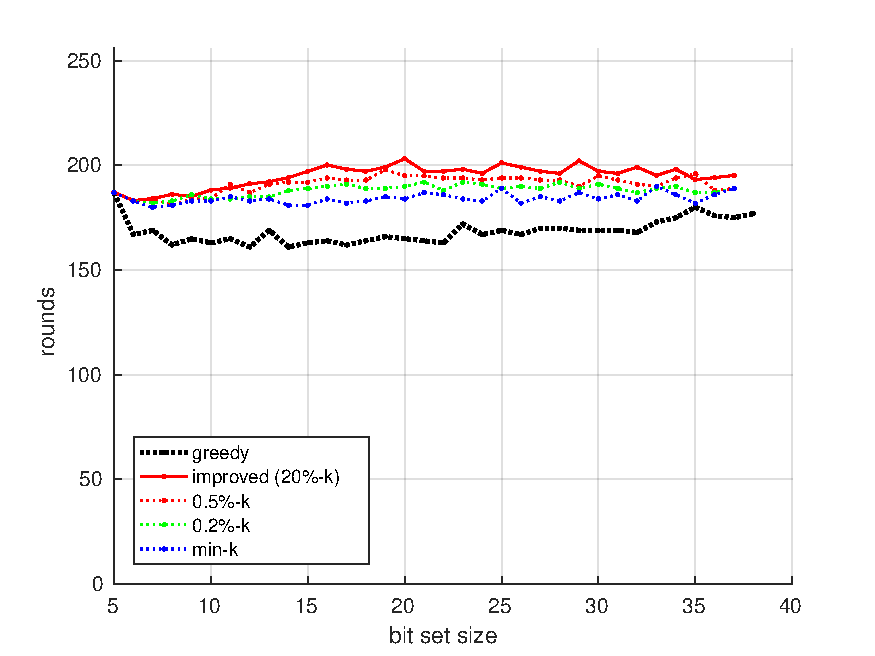
\includegraphics[width=1.07\columnwidth]{kalpha_pres1}
		\captionsetup{singlelinecheck=true}
		\caption{Grain-128a}
		\label{fig:kalphagrain128a}
	\end{subfigure}%
	\begin{subfigure}[b]{0.5\textwidth}
		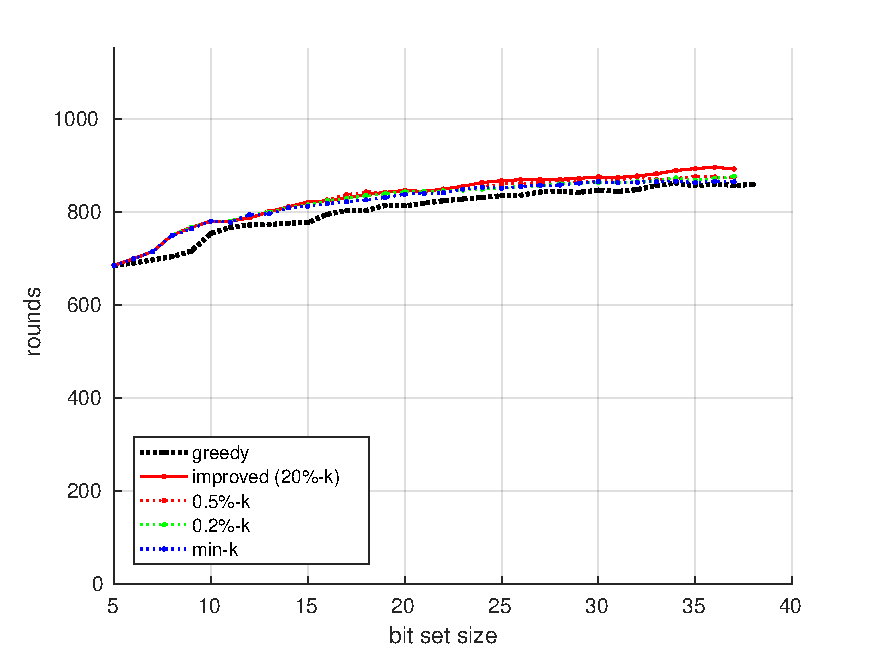
\includegraphics[width=1.07\columnwidth]{kalpha_pres1_kreyvium}
		\captionsetup{singlelinecheck=true}
		\caption{Kreyvium}
		\label{fig:kalphakreyvium}
	\end{subfigure}	
	\caption{Varying $k$ and $\alpha$, with $n_i=1$. Thick dotted black line is the greedy baseline.}
	\label{fig:kalpha}
\end{figure}

\begin{figure}[htbp]
	\centering
	\begin{subfigure}[b]{0.5\textwidth}
		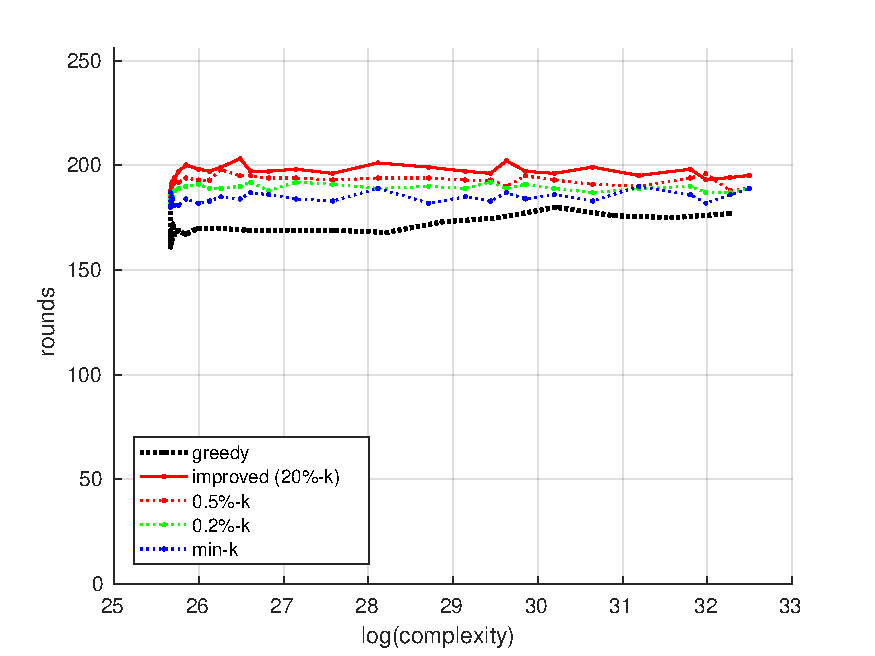
\includegraphics[width=1.07\columnwidth]{kalpha_pres1_complexity}
		\captionsetup{singlelinecheck=true}
		\caption{Grain-128a}
		\label{fig:kalphacomplexitygrain128a}
	\end{subfigure}%
	\begin{subfigure}[b]{0.5\textwidth}
		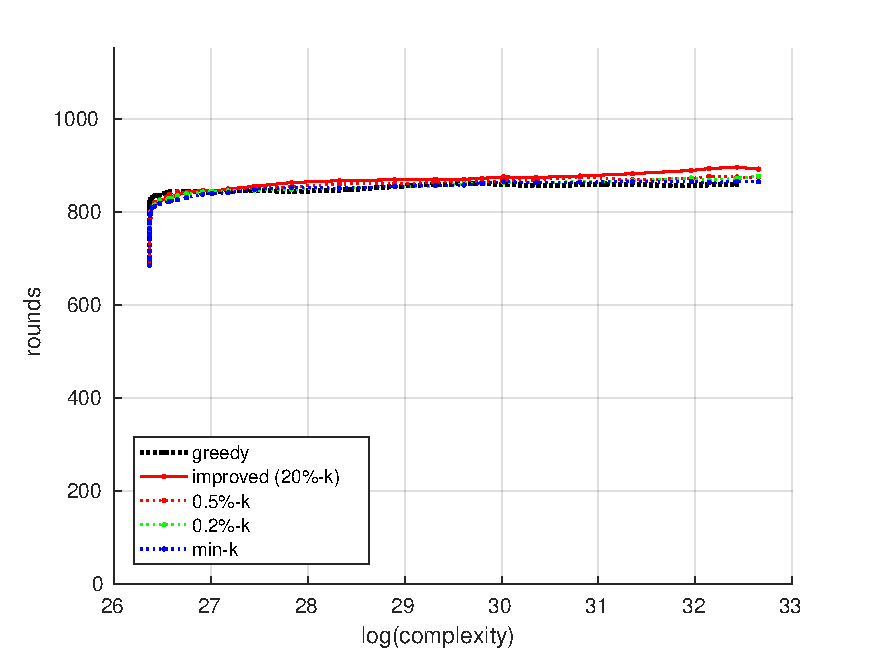
\includegraphics[width=1.07\columnwidth]{kalpha_pres1_kreyvium_complexity}
		\captionsetup{singlelinecheck=true}
		\caption{Kreyvium}
		\label{fig:kalphacomplexitykreyvium}
	\end{subfigure}
	
	\caption{Varying $k$ and $\alpha$, with $n_i=1$. Thick dotted black line is the greedy baseline. The $x$-axis scaled according to logarithmic computational complexity.}
	\label{fig:kalphacomplexity}
\end{figure}

%\subsection{Varying $\bm{n}$}
\subsection{Varying the Number of Bits Added in Each Iteration}

In the previous section, a fixed $\bm{n}$ was used throughout all tests. In this section, we will instead focus on the input parameter vector $\bm{n}$ and see how different vectors affect the result of the algorithm. Recall that this vector decides how many bits that is added to the subset in each iteration.

Intuitively, we expect a higher value of a single $n_i$ to yield better results, since this also reduces the risk to get stuck in a local optima. However, having a large, constant $n_i$ in all iterations, as explored in \cite{stankovski:2010}, means that later iterations will be require very heavy computations. We therefore explore three different variants, where the vector $\bm{n}$ contains decreasing values of $n_i$. These results are then compared to the previous greedy approach where a constant $n$ of different values where used throughout the whole algorithm.

For these tests, the computational complexity will vary between the different tests. This is different from the previous section where the tests were designed to have the same computational complexity. Therefore the results are once again presented in two ways, first as plots where the $x$-axis is the subset size, as seen in \autoref{fig:n}.
The other plots present the results plotted by their computational complexity. As in the last section, the complexity is calculated using \autoref{eq:complexity}, and the plot uses a logarithmic scale on the $x$-axis. This can be seen in \autoref{fig:ncomplexity}. The results for each test case are also available in tabular form in \autoref{tbl:n}.

From the results we note that regardless of our choice of $\bm{n}$, our algorithm outperforms the greedy variants. For Grain-128a, we also see that a higher $n_i$ in the initial iterations seem to lead to better results which remain as the algorithm proceeds towards larger subsets. The results for Kreyvium are not as clear, and it seems like the size of the resulting subset is the most important property.

% allow three consecutive floats.
%\setcounter{topnumber}{3}

\begin{table}[htb]
	\centering
    \caption{Maximum length of initial sequence of zeros in MDM signature when varying $\bm{n}$, expressed as actual count, and percentage of total initialization rounds}
    \begin{tabular}{lrrrr}
    	\toprule
        & \multicolumn{2}{c}{Grain-128a} & \multicolumn{2}{c}{Kreyvium} \\
        \cmidrule(r){2-3} \cmidrule(l){4-5}
                  & Count & Percentage & Count & Percentage \\
        \midrule
        Greedy 1-bit & 187 & 73.1 & 862 & 74.8 \\
        Greedy 2-bit & 187 & 73.1 & 864 & 75.0 \\
        Greedy 3-bit & 187 & 73.1 & 851 & 73.9 \\
        2-2-2-2-2-2-2-2-1-\ldots & 203 & 79.3 & 868 & 75.4 \\
        2-2-2-2-1-\ldots & 199 & 77.7 & 872 & 75.7 \\
        1-\ldots & 195 & 76.2 & 869 & 75.4 \\ 
        \bottomrule
    \end{tabular}
    \label{tbl:n}
\end{table}


\begin{figure}[htbp]
	\centering
	\begin{subfigure}[b]{0.5\textwidth}
		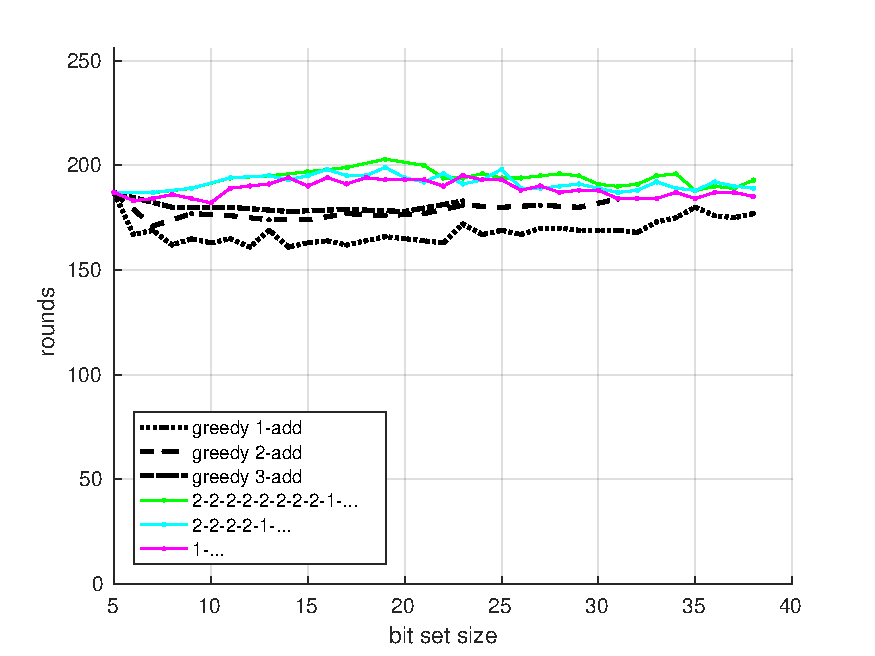
\includegraphics[width=1.07\columnwidth]{nstat_pres}
		\captionsetup{singlelinecheck=true}
		\caption{Grain-128a}
		\label{fig:ngrain128a}
	\end{subfigure}%
	\begin{subfigure}[b]{0.5\textwidth}
		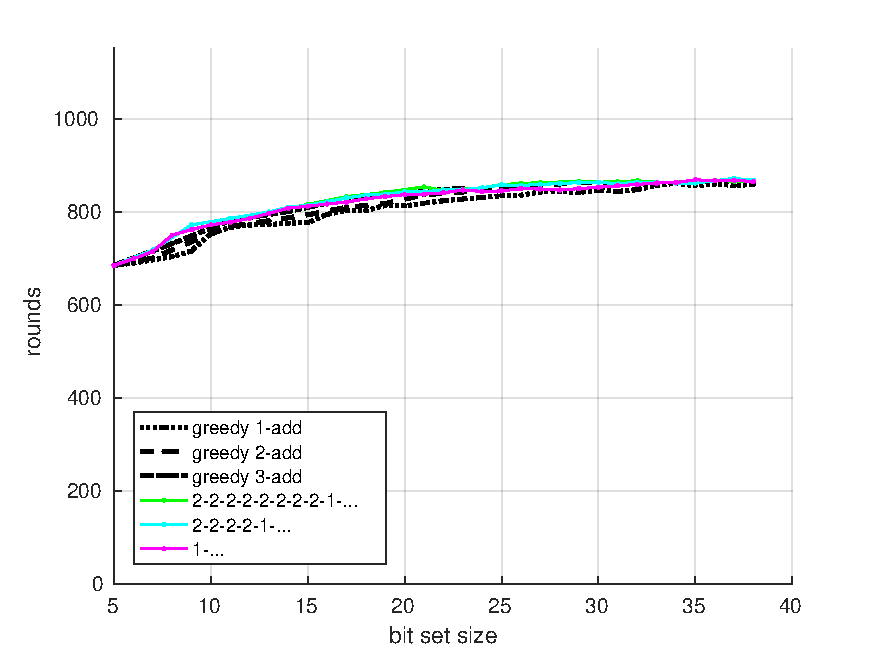
\includegraphics[width=1.07\columnwidth]{nstat_pres_kreyvium}
		\captionsetup{singlelinecheck=true}
		\caption{Kreyvium}
		\label{fig:nkreyvium}
	\end{subfigure}
	
	\caption{Varying $n$. Thick black lines are the greedy baselines for $n$ equal to 1, 2, and 3.}
	\label{fig:n}
\end{figure}

\begin{figure}[htbp]
	\centering
	\begin{subfigure}[b]{0.5\textwidth}
		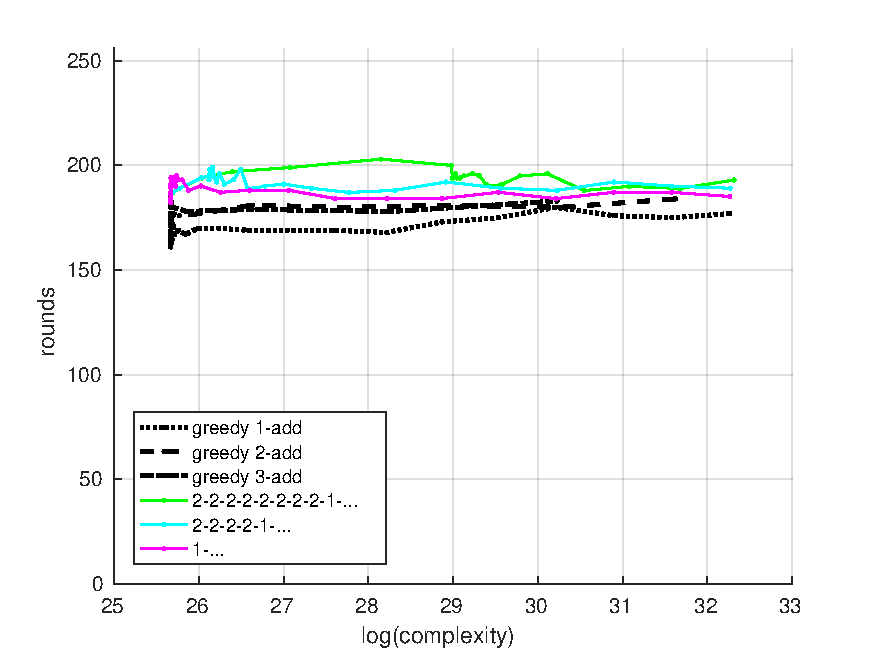
\includegraphics[width=\columnwidth]{nstat_pres_complexity}
		\captionsetup{singlelinecheck=true}
		\caption{Grain-128a}
		\label{fig:ncomplexitygrain128a}
	\end{subfigure}%
	\begin{subfigure}[b]{0.5\textwidth}
		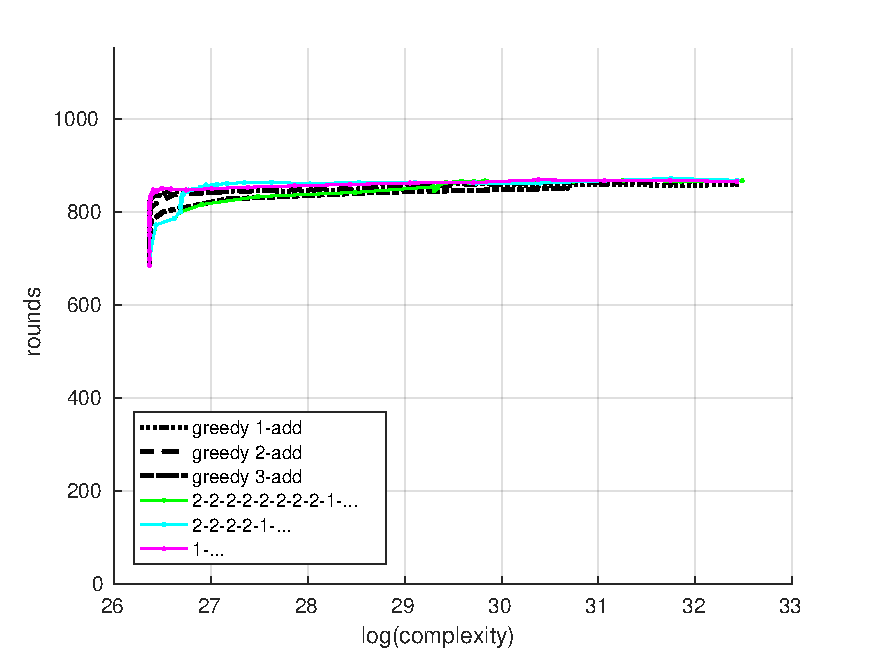
\includegraphics[width=\columnwidth]{nstat_pres_kreyvium_complexity}
		\captionsetup{singlelinecheck=true}
		\caption{Kreyvium}
		\label{fig:ncomplexitykreyvium}
	\end{subfigure}
	
	\caption{Varying $n$. Thick black lines are the greedy baselines for $n$ equal to 1, 2, and 3. The $x$-axis scaled according to logarithmic computational complexity.}
	\label{fig:ncomplexity}
\end{figure}

\subsection{Results for Different Starting Points}

In the previous tests, optimal subsets of size 5 has been used as a starting point for the simulations. In this section, we compare the use of such an optimal start to starting from an empty subset. A simple approach has been chosen, namely to reuse two test cases from \autoref{sec:tuninggreedy}, namely the test case named 20~\%-k for both Grain-128a and Kreyvium. These test cases start with optimal subsets of size 5.

The two new additional test cases start with an empty subset, and then sequentially add one bit during the first five iterations. The remaining  iterations' parameters are kept the same between all test cases, so that the difference in the initial start is isolated. In this way we can investigate whether this optimal starting set is important or not.

The result of this experiment can be found in \autoref{fig:startingset}, again with one subfigure for Grain-128a and one for Kreyvium. The results are summarized in \autoref{tbl:startingset}. In summary, the differences are very small, and for Kreyvium non-existent, which means that the choice of initial starting point may not be the most important decision to make when selecting parameters for the algorithm.

\begin{table}[htb]
	\centering
    \caption{Maximum length of initial sequence of zeros in MDM signature with different starting subsets, expressed as actual count, and percentage of total initialization rounds}
    \begin{tabular}{lrrrr}
    	\toprule
        & \multicolumn{2}{c}{Grain-128a} & \multicolumn{2}{c}{Kreyvium} \\
        \cmidrule(r){2-3} \cmidrule(l){4-5}
                  & Count & Percentage & Count & Percentage \\
        \midrule
        5-bit optimal start & 203 & 79.3 & 896 & 77.8 \\
        Empty subset start & 201 & 78.5 & 896 & 77.8 \\
        \bottomrule
    \end{tabular}
    \label{tbl:startingset}
\end{table}


\begin{figure}[htbp]
	\centering
	\begin{subfigure}[b]{0.5\textwidth}
		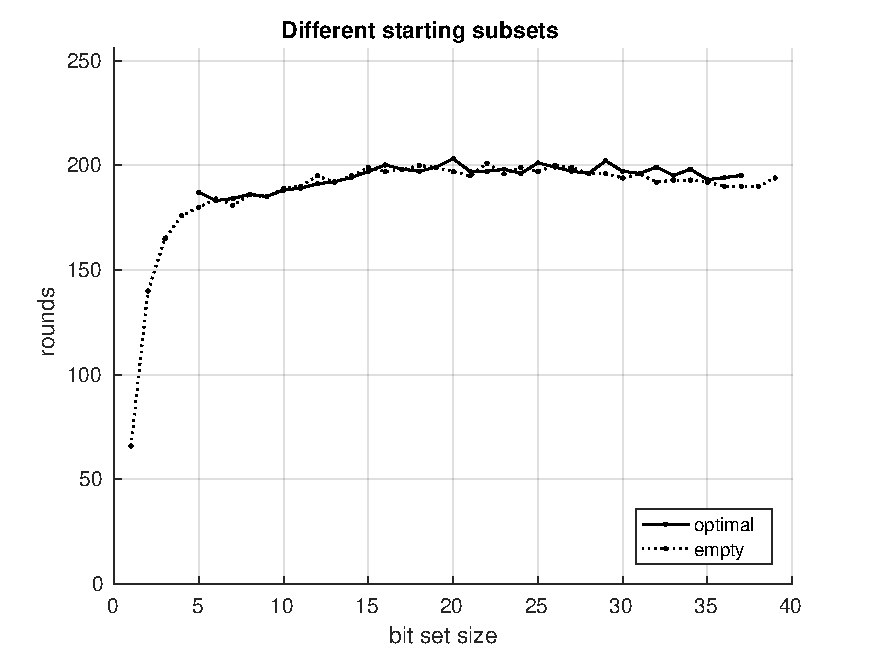
\includegraphics[width=1.07\columnwidth]{startingset_pres_grain128a}
		\captionsetup{singlelinecheck=true}
		\caption{Grain-128a}
		\label{fig:startingsetgrain128a}
	\end{subfigure}%
	\begin{subfigure}[b]{0.5\textwidth}
		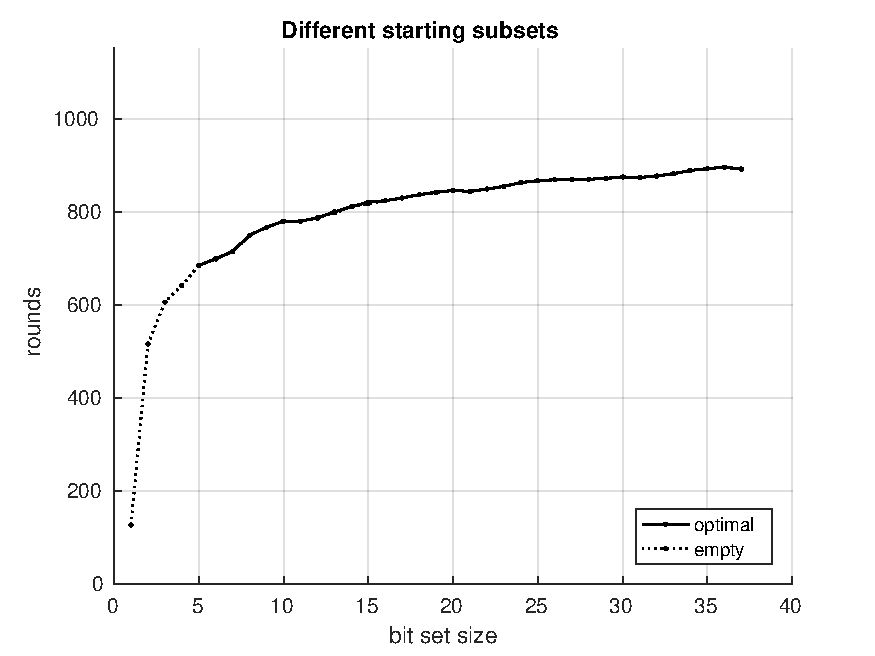
\includegraphics[width=1.07\columnwidth]{startingset_pres_kreyvium}
		\captionsetup{singlelinecheck=true}
		\caption{Kreyvium}
		\label{fig:startingsetkreyvium}
	\end{subfigure}
	
	\caption{Different starting sets and how they affect the results}
	\label{fig:startingset}
\end{figure}

\subsection{Results on Grain-128}
% results for good old grain-128, where we actually found a 256/256 bitset fairly fast.

Apart from new results on Grain-128a and Kreyvium, tests were also performed on Grain-128, a predecessor of Grain-128a which has been analyzed in other works. In \cite{stankovski:2010}, a full-round (256 out of 256 initialization rounds) result was presented using a subset of size 40, using only IV-bits, with an optimal starting subset of size 6. This was found using a constant $n=2$. This corresponds to a parameter set of $\bm{\alpha} = [1.0, 1.0, 1.0, \ldots])$, $\bm{k} = [1, 1, 1, \ldots]$, and $\bm{n} = [6, 2, 2, \ldots]$ in our improved algorithm.

It would clearly be possible to find the exact same subset using our improved algorithm, but we are also interested in seeing whether or not we can find other subsets resulting in full-round results using our improved algorihtm.
A new set of parameters for our improved algorithm is constructed as follows:
The possibility to keep multiple candidates in each step is utilized, especially in the beginning where there are still small subsets. Using the improved algorithm, a smaller subset of size 25 is found, which still gives us a full-round result of 256 out of 256 initialization rounds.

Using the complexity expression in Equation~\ref{eq:complexity}, the computational complexity between the two results can be compared. We find that our improved algorithm has a complexity which is a factor about $2^{12}$ lower than the earlier result, while still finding an equal amount of zeros in the MDM signature.

\section{Related Work} \label{sec:slightlygreedy:relatedwork}

Related work can be divided into two main categories: work related to the maximum degree monomial test, and work related to general cryptanalysis of the discussed ciphers. 

In \cite{saarinen:2006}, Saarinen described the $d$-Monomial test, and how it can be applied in chosen-IV attacks against stream ciphers. In contrast to our work, and the work done by Stankovski \cite{stankovski:2010}, Saarinen considers monomials of various degrees, namely monomials up to degree $d$, therefore the name $d$-Monomial test. In addition to this difference, the choice of input subset bits is different. Saarinen only considers consecutive bits either in the beginning or in the end of the IV. This is in contrast to our work, where the subset is chosen freely as any subset of IV and/or key bits.

Related to the work of Saarinen, the Maximum Degree Monomial (MDM) was introduced by Englund et. al. in \cite{englund:2007}. Rather than looking at several different degrees of monomials, the MDM test only focuses on the maximum degree monomial. The motivation behind this choice is that the maximum degree monomial is likely to occur only if all IV bits have been properly mixed. In addition to this, the existence of the maximum degree monomial is easy to find. The coefficient of the monomial can be found by simply XORing all entries in the truth table.

In the previously mentioned work, a subset of the IV space was used in the tests. In \cite{stankovski:2010}, a greedy heuristic to find these subsets was discussed. The greedy algorithm started with an optimal, precalculated, subset of a small size, and then added $n$ bits in each step in a greedy fashion. In addition, both IV and key bits were suggested for getting distinguisher and nonrandomness results, respectively. Several different ciphers were analyzed, among them Grain-128 and Trivium.

Other work related to distinguishers for Trivium is \cite{liu:2015}, where the authors concentrate on small cubes, and instead look at unions of these cubes. Another difference is that they look at sub-maximal degree monomial tests.

 % from: "Observing biases in the state: case studies with Trivium and Trivia-SC", Santanu Sarkar, Subhamoy Maitra, Anubhab Baksi, 
Also partly based on Stankovski's work is the work in \cite{sarkar:2016}, where the authors propose two new, alternative heuristics. Here, the heuristic is modified so that it does not maximize the initial sequence of zeros in the MDM signature. Rather, in the first heuristic, called ``maximum last zero'', the authors not only maximize the initial sequence of zeros, but also ensure that the position of the current iteration in the MDM signature is a zero as well. In their second heuristic, called ``maximum frequency of zero'', they instead look at the total amount of zeros in the MDM signature. Their heuristics are applied to the ciphers Trivium \cite{canniere:2006} and Trivia-SC \cite{chakraborti:2015}. Similar to our paper, they also mention the use of a non-constant $n$, i.e. a $\bm{n}$-vector, although the authors do not discuss the reasons for this extension.
% they also discuss tie cases, something we e.g. get "for free" in our algorithm as long as k > 1.

In \cite{vielhaber:2007} an attack called AIDA on a modified version of Trivium was presented. In this case Trivium was modified so that it only had half of the original count of initialization rounds. Related to this attack are the 
cube attacks \cite{dinur:2009}, and especially the dynamic cube attack \cite{dinur:2011} which was used to attack Grain-128.

% random attacks in general against grain-128a
Attacks on the newer Grain-128a can be found in the literature as well. In \cite{banik:2013} the authors present a related-key key attack requiring $>2^{32}$ related keys and $>2^{64}$ chosen IVs, while in \cite{sarkar:2014} the authors present a differential fault attack against all the three ciphers in the Grain-family.

% kreyvium analys: (new for extended paper)
There is very limited work regarding the analysis of Kreyvium, possibly because the original Kreyvium paper is relatively recent, however in \cite{watanabe:2017} the authors discuss conditional differential cryptanalysis of Kreyvium.

\section{Conclusions} \label{sec:slightlygreedy:conclusions}

This paper has described the design and motivation of the maximum degree monomial test when designing nonrandomness detectors. The MDM test requires a subset of key and IV bits, and in this paper we have designed and proposed a new algorithm to find such subsets. Our algorithm is based on a greedy approach, but rather than using a na\"{i}ve greedy algorithm, we propose an algorithm which is less likely to get stuck in local optima, and therefore yields better final results. The algorithm is highly flexible, and parameters can be chosen and adapted to get a both reasonable and predictable computational complexity. To validate our algorithm, we have performed a significant amount of simulations to find good input parameters to our algorithm. Simulations has been performed mainly on the ciphers Grain-128a and Kreyvium, and the results show that our new algorithm outperforms previously proposed na\"{i}ve greedy algorithms.

% DONE: rewritten
\section*{Acknowledgments}
This paper is an extended and revised version of the paper ``Improved Greedy Nonrandomness Detectors for Stream Ciphers'' previously presented at ICISSP 2017 \cite{karlsson:2017}.

The computations were performed on resources provided by the Swedish National Infrastructure for Computing (SNIC) at Lunarc.

%\vfill
%\bibliographystyle{splncs03}
%{
%\bibliography{slightlygreedy}}

{\raggedright
	\printbibliography[segment=\therefsegment,heading=subbibliography]
}

% Placed here to allow for top placement of the above table.
\section*{Appendix}%
\addcontentsline{toc}{section}{Appendix}%
\markright{Appendix}

This appendix contains the exact vectors used for the different results discussed in \autoref{sec:results}. The vectors used for the results for varying $\bm{k}$ and $\bm{\alpha}$ are given in \autoref{tbl:appkalpha}. In the same fashion, the vectors used for the results for varying $\bm{n}$ are presented in \autoref{tbl:appn}. Finally, the vectors for the results on Grain-128 are given in \autoref{tbl:appgrain128}.

\begin{table*}[htb]
	\centering
    \caption{Varying $\bm{k}$ and $\bm{\alpha}$ \cite{karlsson:2017}}
    \footnotesize
    \resizebox{\columnwidth}{!}{%
    \begin{tabular}{rp{11cm}}
    	\toprule
         & Greedy \\
        \midrule
        $\bm{k} $ & \{ 1, 1, 1, 1, 1, 1, 1, 1, 1, 1, 1, 1, 1, 1, 1, 1, 1, 1, 1, 1, 1, 1, 1, 1, 1, 1, 1, 1, 1, 1, 1, 1, 1, 1, 1 \} \\
        $\bm{n} $ & \{ 5, 1, 1, 1, 1, 1, 1, 1, 1, 1, 1, 1, 1, 1, 1, 1, 1, 1, 1, 1, 1, 1, 1, 1, 1, 1, 1, 1, 1, 1, 1, 1, 1, 1, 1 \} \\
        $\bm{\alpha}$ & \{ 1, 1, 1, 1, 1, 1, 1, 1, 1, 1, 1, 1, 1, 1, 1, 1, 1, 1, 1, 1, 1, 1, 1, 1, 1, 1, 1, 1, 1, 1, 1, 1, 1, 1, 1 \} \\
        \midrule

        & Improved (20 \%-k) \\
        \midrule
        $\bm{k} $ & \{ 1000, 200, 200, 200, 200, 200, 200, 200, 200, 200, 200, 200, 100, 60, 60, 20, 20, 20, 20, 20, 20, 12, 6, 3, 2, 2, 2, 2, 2, 1, 1, 1, 1 \} \\
        $\bm{n} $ & \{ 5, 1, 1, 1, 1, 1, 1, 1, 1, 1, 1, 1, 1, 1, 1, 1, 1, 1, 1, 1, 1, 1, 1, 1, 1, 1, 1, 1, 1, 1, 1, 1, 1 \} \\
        $\bm{\alpha}$ & \{ 1.0, 0.005, 0.005, 0.005, 0.005, 0.005, 0.005, 0.005, 0.005, 0.005, 0.005, 0.005, 0.005, 0.01, $\frac{1}{60}$, $\frac{1}{60}$, 0.05, 0.05, 0.05, 0.05, 0.05, 0.05, $\frac{1}{12}$, $\frac{2}{15}$, 0.375, 0.5, 0.5, 0.5, 0.5, $\frac{2}{9}$, 1.0, 0.5, 1.0 \} \\
        \midrule

        & 0.5 \%-k \\
        \midrule
        $\bm{k} $ & \{ 1000, 5, 5, 5, 5, 5, 5, 5, 5, 5, 5, 5, 3, 2, 2, 1, 1, 1, 1, 1, 1, 1, 1, 1, 1, 1, 1, 1, 1, 1, 1, 1, 1 \} \\
        $\bm{n} $ & \{    5, 1, 1, 1, 1, 1, 1, 1, 1, 1, 1, 1, 1, 1, 1, 1, 1, 1, 1, 1, 1, 1, 1, 1, 1, 1, 1, 1, 1, 1, 1, 1, 1 \}  \\
        $\bm{\alpha}$ & \{ 1.0, 0.2, 0.2, 0.2, 0.2, 0.2, 0.2, 0.2, 0.2, 0.2, 0.2, 0.2, $\frac{1}{6}$, 0.3, 0.5, $\frac{1}{3}$, 1.0, 1.0, 1.0, 1.0, 1.0, 0.6, 0.5, 0.4, 0.75, 1.0, 1.0, 1.0, 1.0, $\frac{2}{9}$, 1.0, 0.5, 1.0 \} \\
        \midrule

        & 0.2 \%-k \\
        \midrule
        $\bm{k} $ & \{ 1000, 2, 2, 2, 2, 2, 2, 2, 2, 2, 2, 2, 1, 1, 1, 1, 1, 1, 1, 1, 1, 1, 1, 1, 1, 1, 1, 1, 1, 1, 1, 1, 1 \} \\
        $\bm{n} $ & \{ 5, 1, 1, 1, 1, 1, 1, 1, 1, 1, 1, 1, 1, 1, 1, 1, 1, 1, 1, 1, 1, 1, 1, 1, 1, 1, 1, 1, 1, 1, 1, 1, 1 \} \\
        $\bm{\alpha}$ & \{ 1.0, 0.5, 0.5, 0.5, 0.5, 0.5, 0.5, 0.5, 0.5, 0.5, 0.5, 0.5, 0.5, 0.6, 1.0, $\frac{1}{3}$, 1.0, 1.0, 1.0, 1.0, 1.0, 0.6, 0.5, 0.4, 0.75, 1.0, 1.0, 1.0, 1.0, $\frac{2}{9}$, 1.0, 0.5, 1.0 \}  \\
        \midrule

        & min-k \\
        \midrule
        $\bm{k} $ & \{ 1000, 1, 1, 1, 1, 1, 1, 1, 1, 1, 1, 1, 1, 1, 1, 1, 1, 1, 1, 1, 1, 1, 1, 1, 1, 1, 1, 1, 1, 1, 1, 1, 1 \} \\
        $\bm{n} $ & \{ 5, 1, 1, 1, 1, 1, 1, 1, 1, 1, 1, 1, 1, 1, 1, 1, 1, 1, 1, 1, 1, 1, 1, 1, 1, 1, 1, 1, 1, 1, 1, 1, 1 \} \\
        $\bm{\alpha}$ & \{ 1.0, 1.0, 1.0, 1.0, 1.0, 1.0, 1.0, 1.0, 1.0, 1.0, 1.0, 1.0, 0.5, 0.6, 1.0, $\frac{1}{3}$, 1.0, 1.0, 1.0, 1.0, 1.0, 0.6, 0.5, 0.4, 0.75, 1.0, 1.0, 1.0, 1.0, $\frac{2}{9}$, 1.0, 0.5, 1.0 \}  \\
        \bottomrule
    \end{tabular}%
	}
    \label{tbl:appkalpha}
\end{table*}

\begin{table*}[tbp]
	\centering
    \caption{Varying $\bm{n}$ \cite{karlsson:2017}}
    \footnotesize
    \resizebox{\columnwidth}{!}{%
    \begin{tabular}{rp{11.1cm}}
    	\toprule
         & Greedy 1-add\\
        \midrule
        $\bm{k} $ &     \{ 1, 1, 1, 1, 1, 1, 1, 1, 1, 1, 1, 1, 1, 1, 1, 1, 1, 1, 1, 1, 1, 1, 1, 1, 1, 1, 1, 1, 1, 1, 1, 1, 1, 1, 1 \} \\
        $\bm{n} $ &     \{ 5, 1, 1, 1, 1, 1, 1, 1, 1, 1, 1, 1, 1, 1, 1, 1, 1, 1, 1, 1, 1, 1, 1, 1, 1, 1, 1, 1, 1, 1, 1, 1, 1, 1, 1 \} \\
        $\bm{\alpha}$ & \{ 1, 1, 1, 1, 1, 1, 1, 1, 1, 1, 1, 1, 1, 1, 1, 1, 1, 1, 1, 1, 1, 1, 1, 1, 1, 1, 1, 1, 1, 1, 1, 1, 1, 1, 1 \}  \\
        \midrule

        & Greedy 2-add \\
        \midrule
        $\bm{k} $ & \{ 1, 1, 1, 1, 1, 1, 1, 1, 1, 1, 1, 1, 1, 1 \} \\
        $\bm{n} $ & \{ 5, 2, 2, 2, 2, 2, 2, 2, 2, 2, 2, 2, 2, 2 \} \\
        $\bm{\alpha}$ & \{ 1, 1, 1, 1, 1, 1, 1, 1, 1, 1, 1, 1, 1, 1 \} \\
        \midrule

        & Greedy 3-add \\
        \midrule
        $\bm{k} $ & \{ 1, 1, 1, 1, 1, 1, 1 \} \\
        $\bm{n} $ & \{ 5, 3, 3, 3, 3, 3, 3 \} \\
        $\bm{\alpha}$ & \{ 1, 1, 1, 1, 1, 1, 1 \} \\
       
       \midrule
        & 2-2-2-2-2-2-2-2-1-... \\
        \midrule
        $\bm{k} $ & \{ 1000, 200, 200, 200, 200, 150, 50, 50, 50, 30, 15, 6, 5, 5, 5, 5, 5, 1, 1, 1, 1, 1, 1, 1, 1, 1 \} \\
        $\bm{n} $ & \{ 5, 2, 2, 2, 2, 2, 2, 2, 2, 1, 1, 1, 1, 1, 1, 1, 1, 1, 1, 1, 1, 1, 1, 1, 1, 1 \}  \\
        $\bm{\alpha}$ & \{ 1.0, 0.005, 0.005, 0.0005, 0.005, $\frac{1}{150}$, 0.02,  0.01, 0.02, 0.02, $\frac{1}{15}$,  $\frac{1}{15}$, 0.15, 0.2, 0.2, $\frac{4}{45}$, 0.1, 0.5, 1.0, 1.0, 1.0, 1.0, 1.0, 1.0, 1.0, 1.0 \} \\
       
       \midrule
        & 2-2-2-2-1-... \\
        \midrule
        $\bm{k} $ & \{ 1000, 200, 200, 200, 200, 150, 50, 50, 50, 30, 15, 6, 5, 5, 5, 5, 5, 1, 1, 1, 1, 1, 1, 1, 1, 1, 1, 1, 1, 1 \} \\
        $\bm{n} $ & \{ 5, 2, 2, 2, 2, 1, 1, 1, 1, 1, 1, 1, 1, 1, 1, 1, 1, 1, 1, 1, 1, 1, 1, 1, 1, 1, 1, 1, 1, 1 \} \\
        $\bm{\alpha}$ & \{ 1.0, 0.005, 0.005, 0.0005, 0.005, $\frac{1}{150}$, 0.02, 0.01, 0.02, 0.02, $\frac{1}{15}$, $\frac{1}{15}$, 0.15, 0.2, 0.2, $\frac{4}{45}$, 0.1, 0.5, 1.0, 1.0, 1.0, 1.0, 1.0, 1.0, 1.0, 1.0, 1.0, 1.0, 1.0, 1.0 \}  \\
        
        \midrule
        & 1-... \\
        \midrule
        $\bm{k} $ & \{ 1000, 200, 200, 200, 200, 150, 50, 50, 50, 30, 15, 6, 5, 5, 5, 5, 5, 1, 1, 1, 1, 1, 1, 1, 1, 1, 1, 1, 1, 1, 1, 1, 1, 1 \} \\
        $\bm{n} $ & \{ 5, 1, 1, 1, 1, 1, 1, 1, 1, 1, 1, 1, 1, 1, 1, 1, 1, 1, 1, 1, 1, 1, 1, 1, 1, 1, 1, 1, 1, 1, 1, 1, 1, 1 \}  \\
        $\bm{\alpha}$ & \{ 1.0, 0.005, 0.005, 0.0005, 0.005, $\frac{1}{150}$, 0.02, 0.01, 0.02, 0.02, $\frac{1}{15}$, $\frac{1}{15}$, 0.15, 0.2, 0.2, $\frac{4}{45}$, 0.1, 0.5, 1.0, 1.0, 1.0, 1.0, 1.0, 1.0, 1.0, 1.0, 1.0, 1.0, 1.0, 1.0, 1.0, 1.0, 1.0, 1.0 \} \\
        \bottomrule
    \end{tabular}%
	}
    \label{tbl:appn}
\end{table*}

\begin{table*}[p]
	\centering
    \caption{Results on Grain-128 \cite{karlsson:2017}}
    \footnotesize
    \resizebox{\columnwidth}{!}{%
    \begin{tabular}{rp{11.1cm}}
    	\toprule
         & Greedy 1-add\\
        \midrule
        $\bm{k} $ &  \{ 1000, 80, 80, 80, 80, 80, 80, 80, 80, 80, 80, 80, 80, 60, 60, 20, 20, 20, 20, 20 \}    \\
        $\bm{n} $ &  \{ 6, 1, 1, 1, 1, 1, 1, 1, 1, 1, 1, 1, 1, 1, 1, 1, 1, 1, 1, 1 \}    \\
        $\bm{\alpha}$ & \{ 1.0, 0.0125, 0.0125, 0.0125, 0.0125, 0.0125, 0.0125, 0.0125, 0.0125, 0.0125, 0.0125, 0.0125, 0.00625, 0.01, $\frac{1}{60}$, $\frac{1}{60}$, 0.05, 0.05, 0.05, 0.05 \}  \\
        \bottomrule
    \end{tabular}%
	}
    \label{tbl:appgrain128}
\end{table*}

}